\documentclass[xcolor=x11names,compress,professionalfonts]{beamer}

%% General packages %%%%%%%%%%%%%%%%%%%%%%%%%%%%%%%%%%
\usepackage[utf8]{inputenc}
\usepackage{graphicx}
\usepackage{tikz}
\tikzset{% change default arrow tips
    >=latex
}
\usepackage{ifthen}

\usepackage{amsmath}
\usepackage{nicefrac}

\usepackage{color}

%%%%%%%%%%%%%%%%%%%%%%%%%%%%%%%%%%%%%%%%%%%%%%%%%%%%%%


%% Beamer Layout %%%%%%%%%%%%%%%%%%%%%%%%%%%%%%%%%%
\useoutertheme[subsection=false,shadow]{miniframes}
\useinnertheme{rectangles}

\setbeamertemplate{navigation symbols}{}%remove navigation symbols

\usepackage{libertine}
\usepackage[T1]{fontenc}

\setbeamerfont{title like}{shape=\scshape}
\setbeamerfont{frametitle}{shape=\scshape}

\setbeamercolor*{lower separation line head}{bg=DeepSkyBlue4} 
\setbeamercolor*{normal text}{fg=black,bg=white} 
\setbeamercolor*{alerted text}{fg=red} 
\setbeamercolor*{example text}{fg=black} 
\setbeamercolor*{structure}{fg=black} 
 
\setbeamercolor*{palette tertiary}{fg=black,bg=black!10} 
\setbeamercolor*{palette quaternary}{fg=black,bg=black!10} 

\renewcommand{\(}{\begin{columns}}
\renewcommand{\)}{\end{columns}}
\newcommand{\<}[1]{\begin{column}{#1}}
\renewcommand{\>}{\end{column}}

\definecolor{BostonBlue}{HTML}{00688B}
\definecolor{Complementary}{HTML}{8B2300}
%%%%%%%%%%%%%%%%%%%%%%%%%%%%%%%%%%%%%%%%%%%%%%%%%%

\usepackage{braket}

%%%My Math

\newcommand{\pd}[2]{\frac{\displaystyle \partial #1}{\displaystyle\partial #2}} % for partial derivatives
\newcommand{\dx}{\mathrm{d}x}
\renewcommand{\d}[1]{\mathrm{d}#1}
\newcommand{\nth}{$n^\text{th}$ }

\newcommand{\mean}[1]{\langle #1 \rangle}
\DeclareMathOperator{\Pf}{Pf}
\DeclareMathOperator{\Tr}{Tr}

\begin{document}


\begin{frame}
\title{Fractals in physics}
%\subtitle{SUBTITLE}
\author{ Nicolas Macé }
\date{
	February 27, 2020
}
\titlepage
\end{frame}

\section{Symmetry}
\subsection{Dummy}

\begin{frame}{Continuous translation symmetry}

Setup: observer $O$ in (empty) space

{
\centering
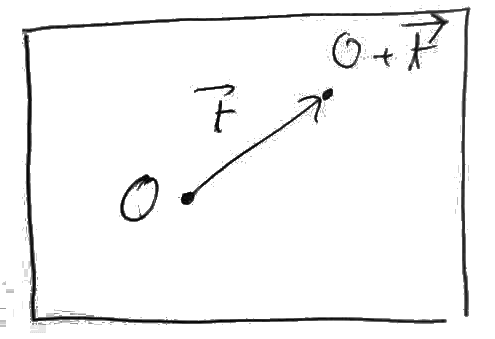
\includegraphics[width=0.4\textwidth]{0_continuous_translation}

}

\begin{itemize}
	\item Translated observer $O + \overrightarrow{t}$ makes the same observations as $O$
	\item $\implies$ \textcolor{BostonBlue}{Continuous} translation symmetry
	\item Formally: $\textcolor{BostonBlue}{\forall \overrightarrow{t}}, O + \overrightarrow{t} \sim O$
\end{itemize}
\end{frame}

\begin{frame}{Symmetry breaking}

Add a reference point $P$

{
\centering
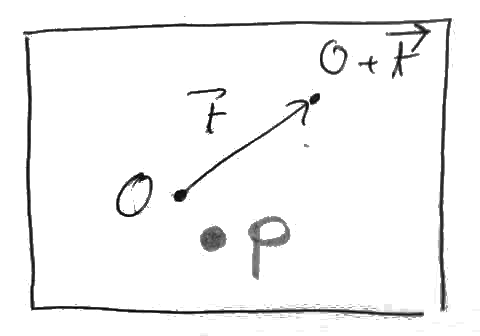
\includegraphics[width=0.4\textwidth]{1_continuous_translation_breaking}

}

\begin{itemize}
	\item Observer can measure distance to $P$: $O + \overrightarrow{t} \not\sim O$
	\item $\implies$ $P$ breaks the symmetry
\end{itemize}

\end{frame}

\begin{frame}{Discrete translation symmetry}

Can we partially restore translation symmetry?

$\to$ add a lattice of reference points

{
\centering
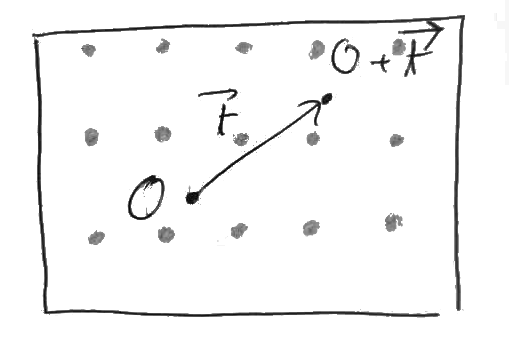
\includegraphics[width=0.4\textwidth]{2_discrete_translation}

}

\begin{itemize}
	\item $\textcolor{Complementary}{\exists \overrightarrow{t}}, O + \overrightarrow{t} \sim O$
	\item $\implies$ \textcolor{Complementary}{Discrete} translation symmetry
\end{itemize}

\end{frame}

\begin{frame}{Continuous scaling symmetry}

Back to empty space:

{
\centering
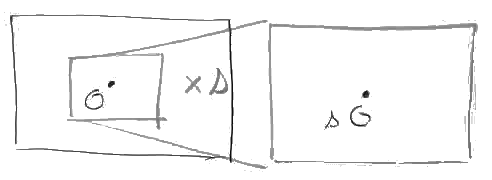
\includegraphics[width=0.7\textwidth]{3_continuous_scaling}

}

\begin{itemize}
	\item Rescaled observer $s O$ makes the same observations as $O$
	\item \textcolor{BostonBlue}{Continuous} scaling symmetry
	\item $\textcolor{BostonBlue}{\forall s}, s O \sim O$
\end{itemize}

Can we break \textcolor{BostonBlue}{continuous} scaling symmetry into \textcolor{Complementary}{discrete}?

\end{frame}

\begin{frame}{Fractals}

{
\centering
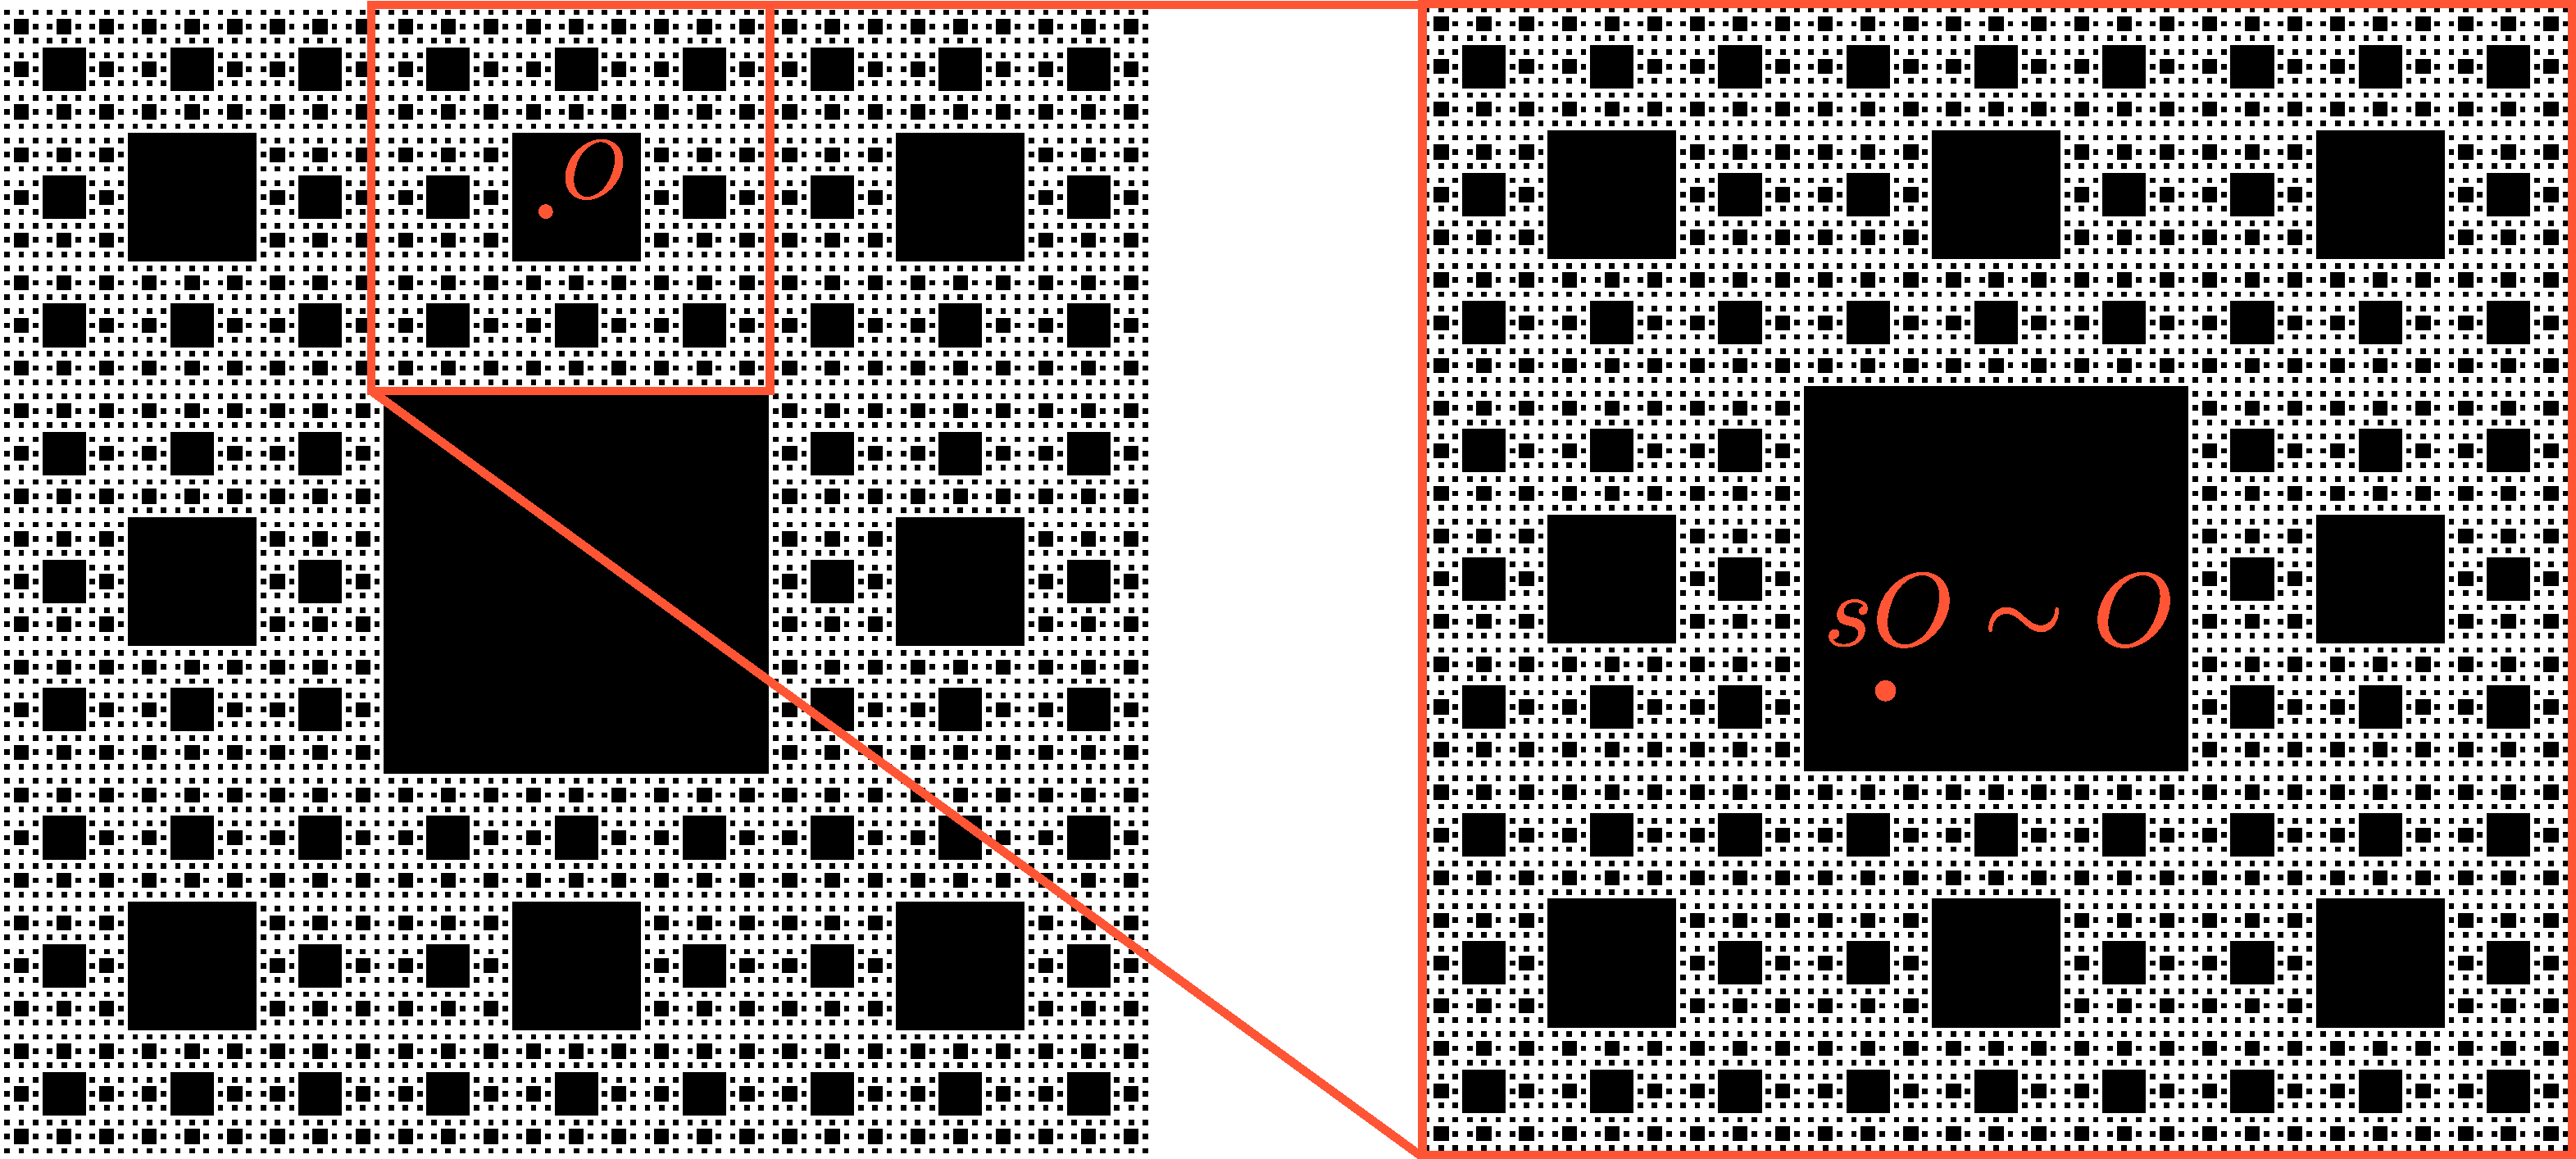
\includegraphics[width=0.6\textwidth]{Sierpinski_carpet_rescaling}

\scriptsize [Menger sponge]

}
\begin{itemize}
	\item \textcolor{Complementary}{Discrete} scaling symmetry: $\textcolor{Complementary}{\exists s}, sO\sim O$ (Menger sponge: $s = 3$)
	\item Fractals: discretely scale invariant objects
	\item $\implies$ fractals: \textbf{rough} objects
\end{itemize}

{
\centering
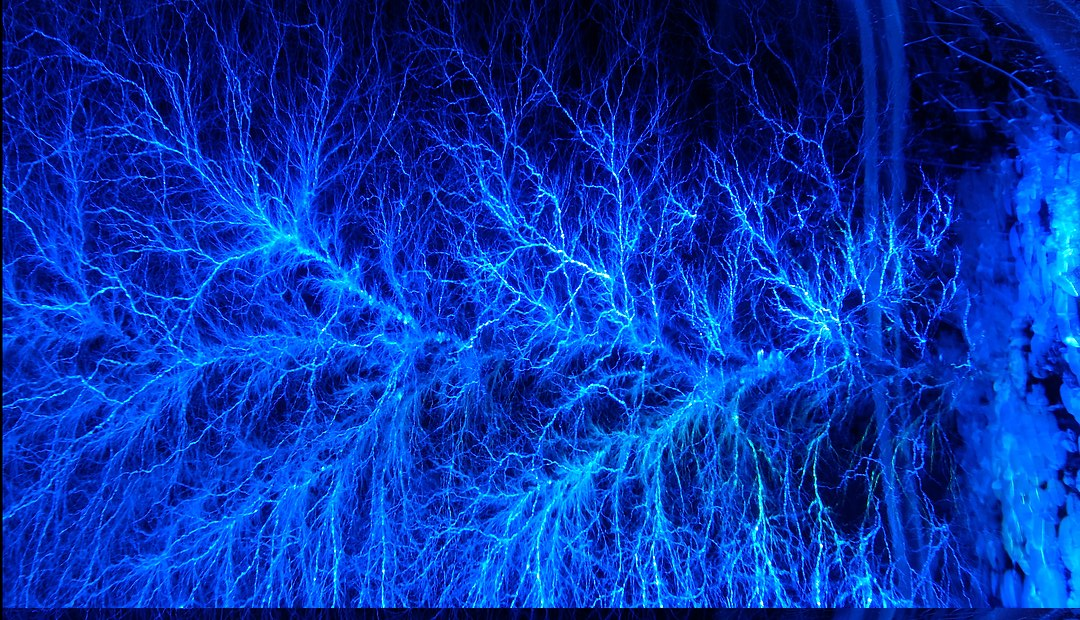
\includegraphics[width=0.4\textwidth]{Lichtenberg-Figur}

\scriptsize [Lichtenberg figure]

}
\end{frame}

\begin{frame}{Symmetry: recap}
    \begin{itemize}
        \item Empty space: continuous translation symmetry \& continuous scaling symmetry
            \begin{itemize}
                \item Lattice: discrete translational symmetry
                \item Fractal: discrete scaling symmetry
            \end{itemize}
    \end{itemize}
    
    $\rightarrow$ fractal: infinitely divisible object
    
    {
    
    \centering
    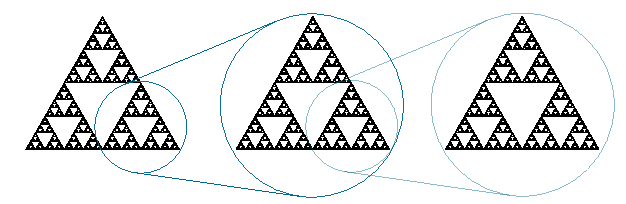
\includegraphics[scale=1.00]{sierpinski.pdf}
    \scriptsize
    
    [Sierpiński triangle]
    
    }
\end{frame}

\section{Geometry}
%Each section needs a subsection for the small points on top to show up
\subsection{Dummy}

\begin{frame}{Geometric construction}{A first example: the Sierpiński triangle}

\begin{itemize} 

\begin{columns}
\newcommand{\s}{.2}
  \begin{column}{3cm}
    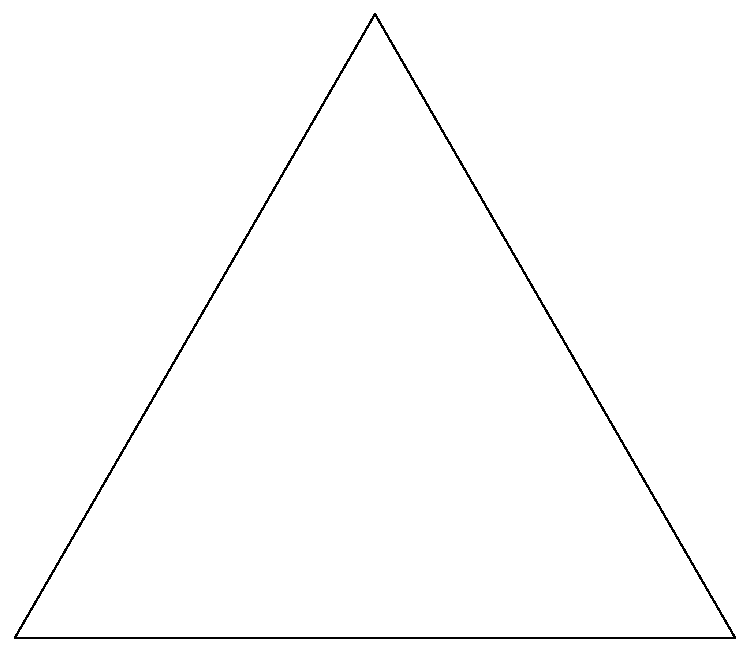
\includegraphics[scale=\s]{sierpinski0.pdf}
  \end{column}

  \begin{column}{3cm}
     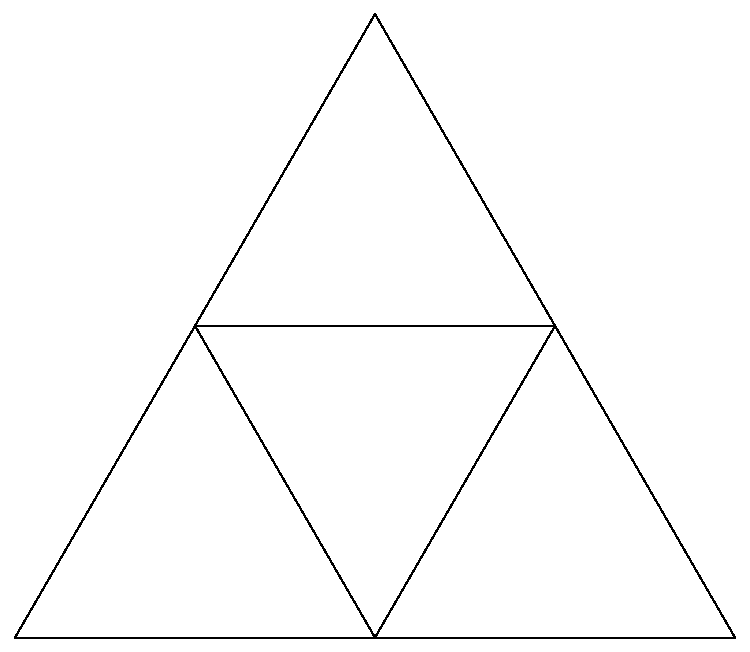
\includegraphics[scale=\s]{sierpinski1.pdf}
  \end{column}
  
  \begin{column}{3cm}
    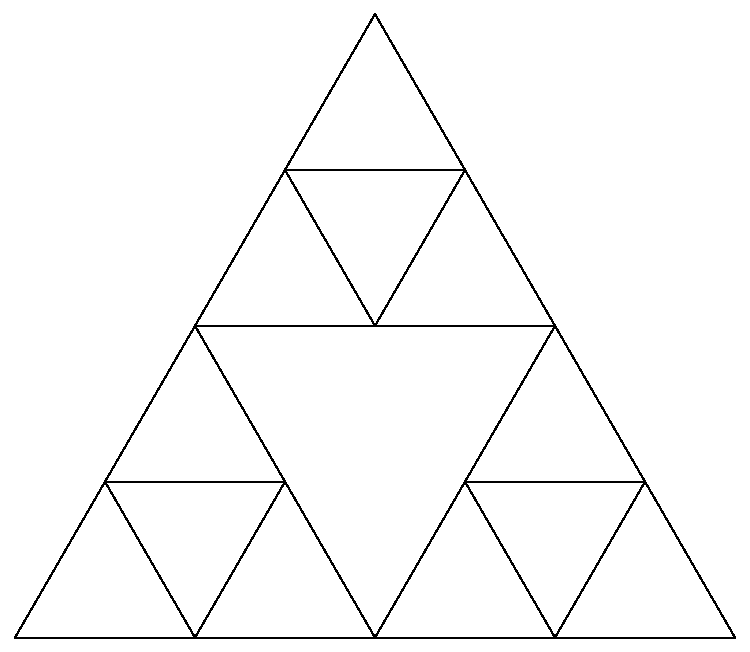
\includegraphics[scale=\s]{sierpinski2.pdf}
  \end{column}
  ...
    \begin{column}{3cm}
    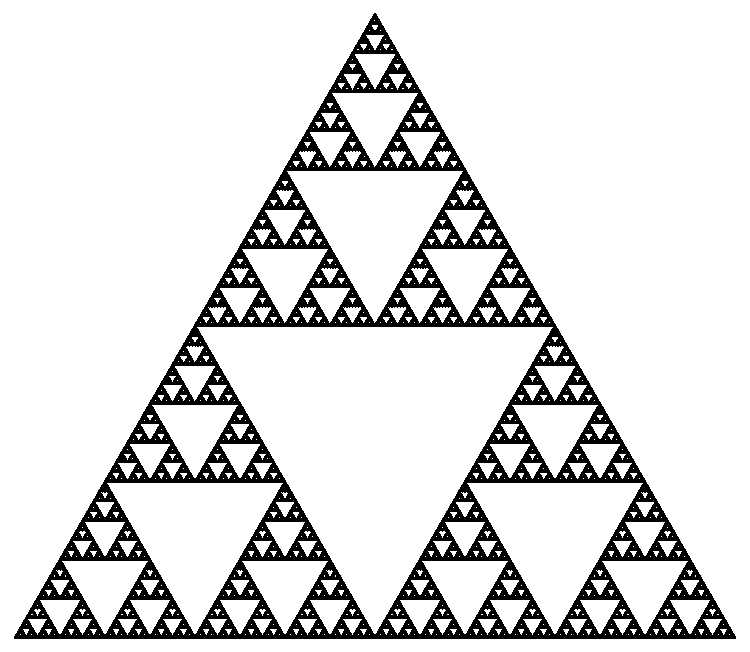
\includegraphics[scale=\s]{sierpinskiInfty.pdf}
  \end{column}
\end{columns}

 	\item independant of starting shape $\rightarrow$ only determined by the geometrical transformations used.

\begin{columns}
\newcommand{\s}{.2}
  \begin{column}{3cm}
    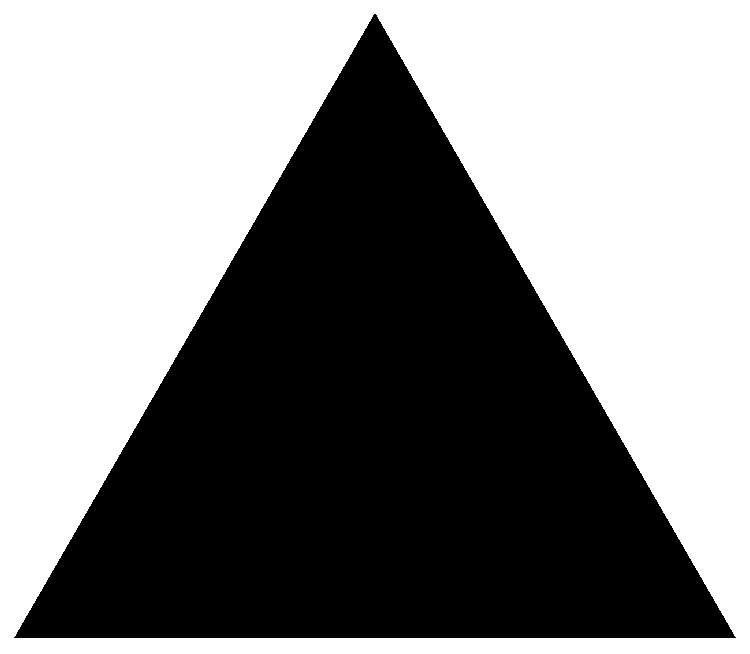
\includegraphics[scale=\s]{sierpinksi_triangle_0}
  \end{column}

  \begin{column}{3cm}
     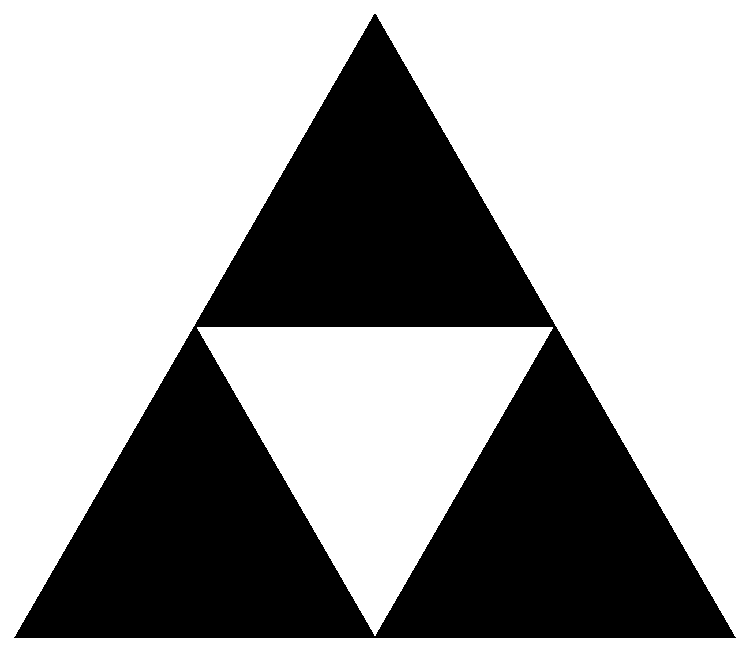
\includegraphics[scale=\s]{sierpinksi_triangle_1}
  \end{column}
  
  \begin{column}{3cm}
    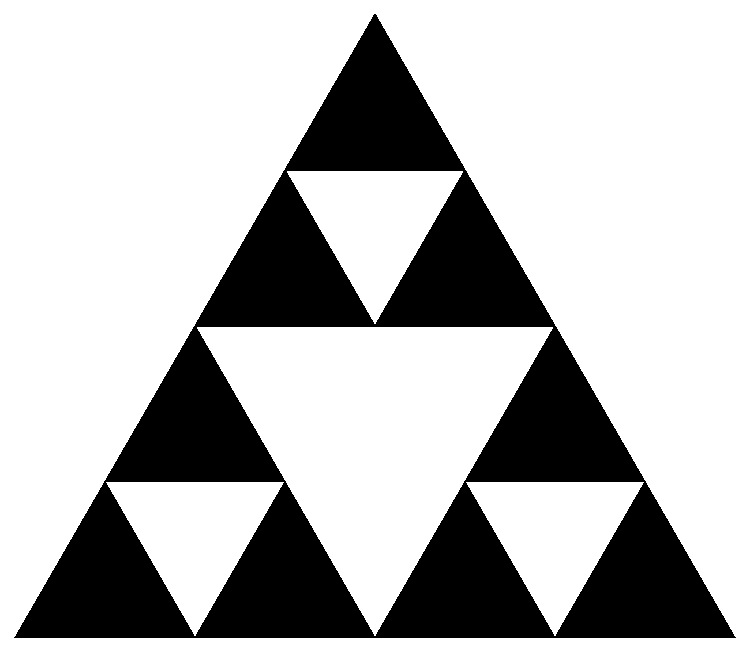
\includegraphics[scale=\s]{sierpinksi_triangle_2}
  \end{column}
  ...
    \begin{column}{3cm}
    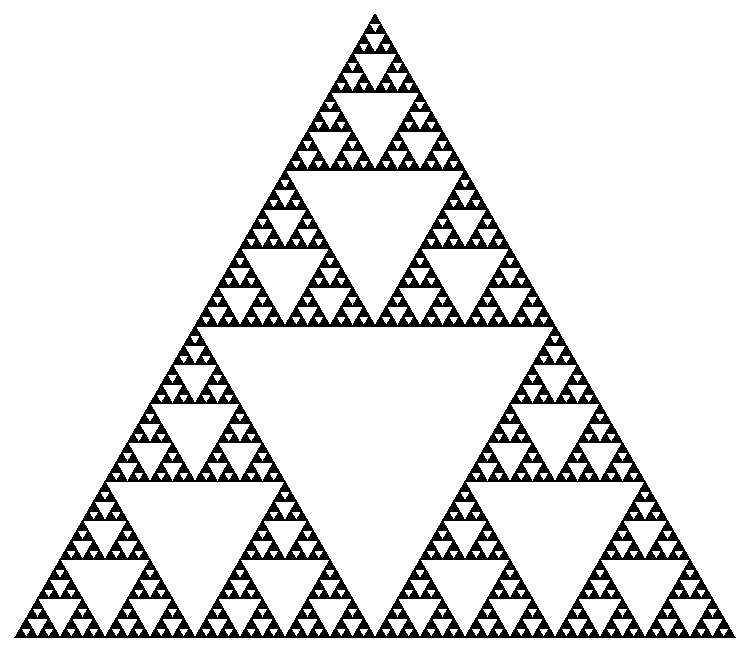
\includegraphics[scale=\s]{sierpinksi_triangle_6}
  \end{column}
\end{columns}

	\item The Sierpiński triangle is constructed by an Iterated Function System (IFS).
\end{itemize}

\end{frame}

\begin{frame}{Geometric construction}{Iterated function systems}

\begin{columns}
\newcommand{\s}{.2}

  \begin{column}{1.5cm}
  \centering
    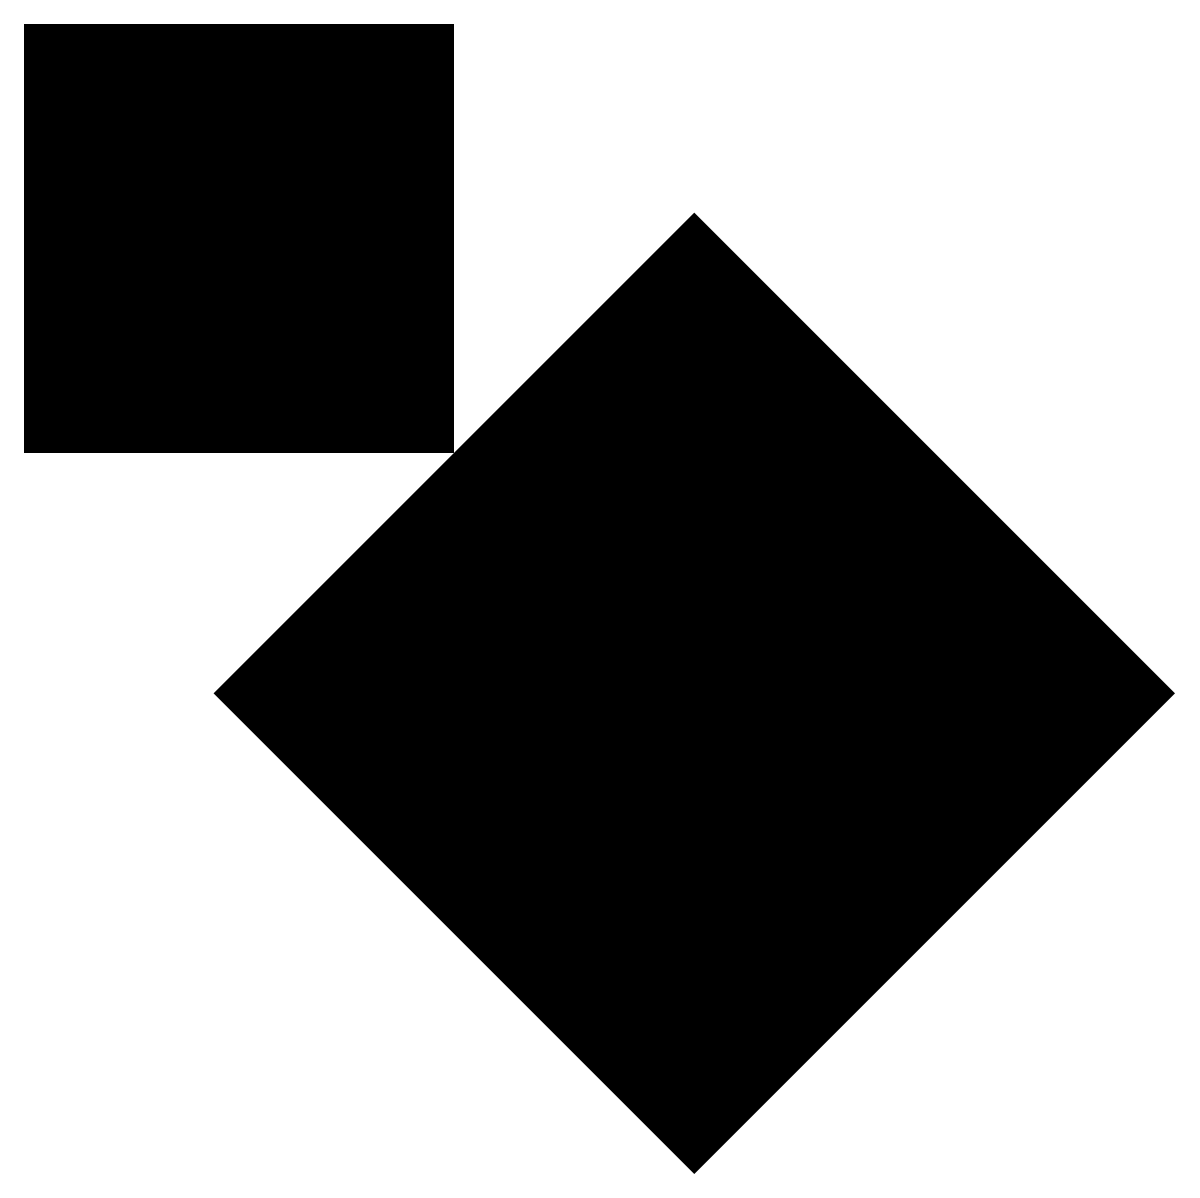
\includegraphics[scale=0.04]{leaf1.png}
  \end{column}

  \begin{column}{3cm}
  \centering
    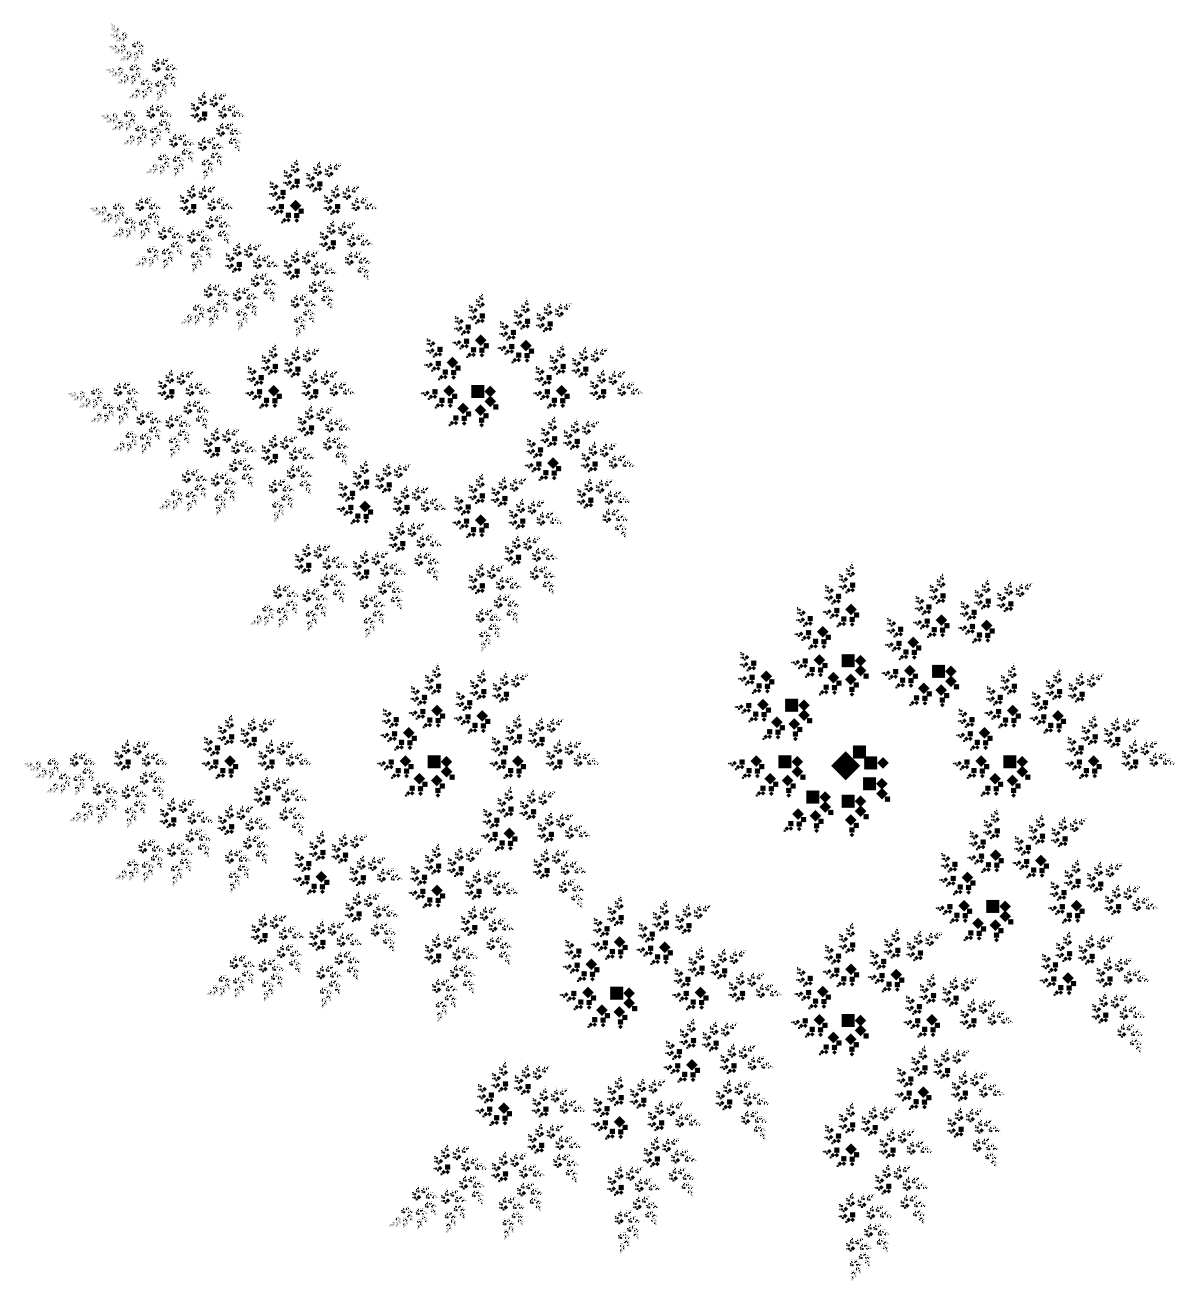
\includegraphics[scale=0.08]{leaf.png}
  \end{column}

  \begin{column}{3cm}
  \centering
     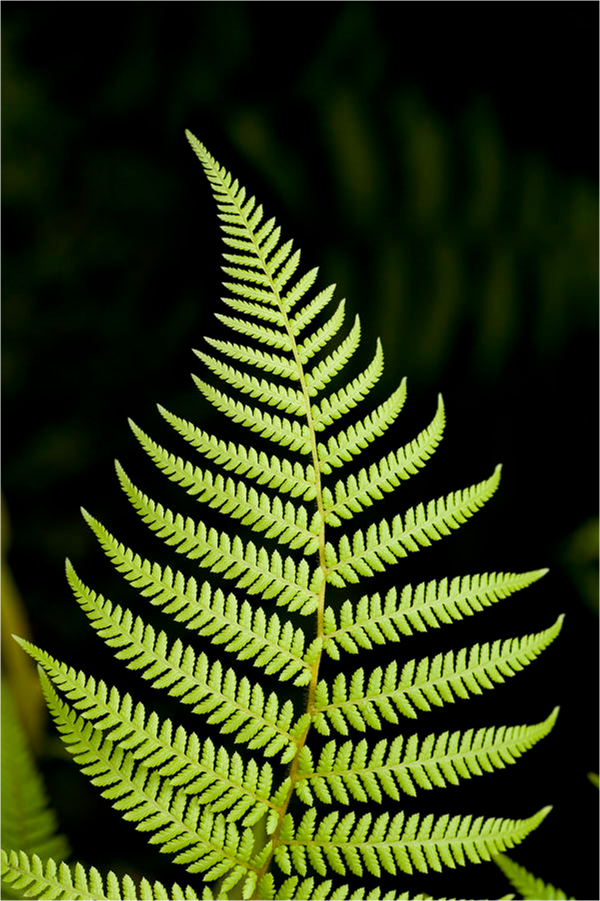
\includegraphics[scale=.4]{fern.png}
  \end{column}
\end{columns}

\begin{itemize}
	\item Every fractal is approached by an IFS [Barnsley 1988].
\end{itemize}

\end{frame}

\begin{frame}{Geometric construction}{``non-trivial'' fractals: Julia sets}
\begin{itemize}
	\item Define a recurrence $z_{n+1} = z_n^2 + c$
	\item (filled) Julia set: set of non-escaping points
\end{itemize}

\centering
\only<1>{
	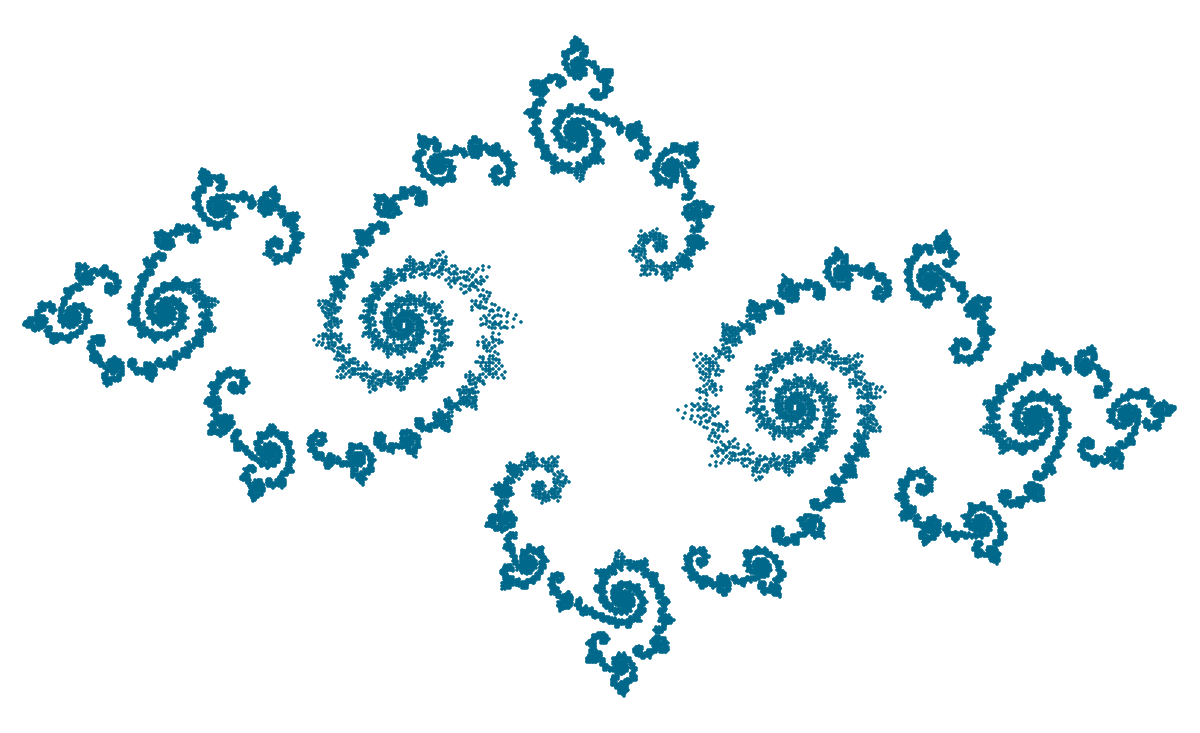
\includegraphics[scale=0.2]{julia.png}
	
	\scriptsize
	    Julia set $c = -0.77 + 0.22 i$
}
    
\only<2>{
	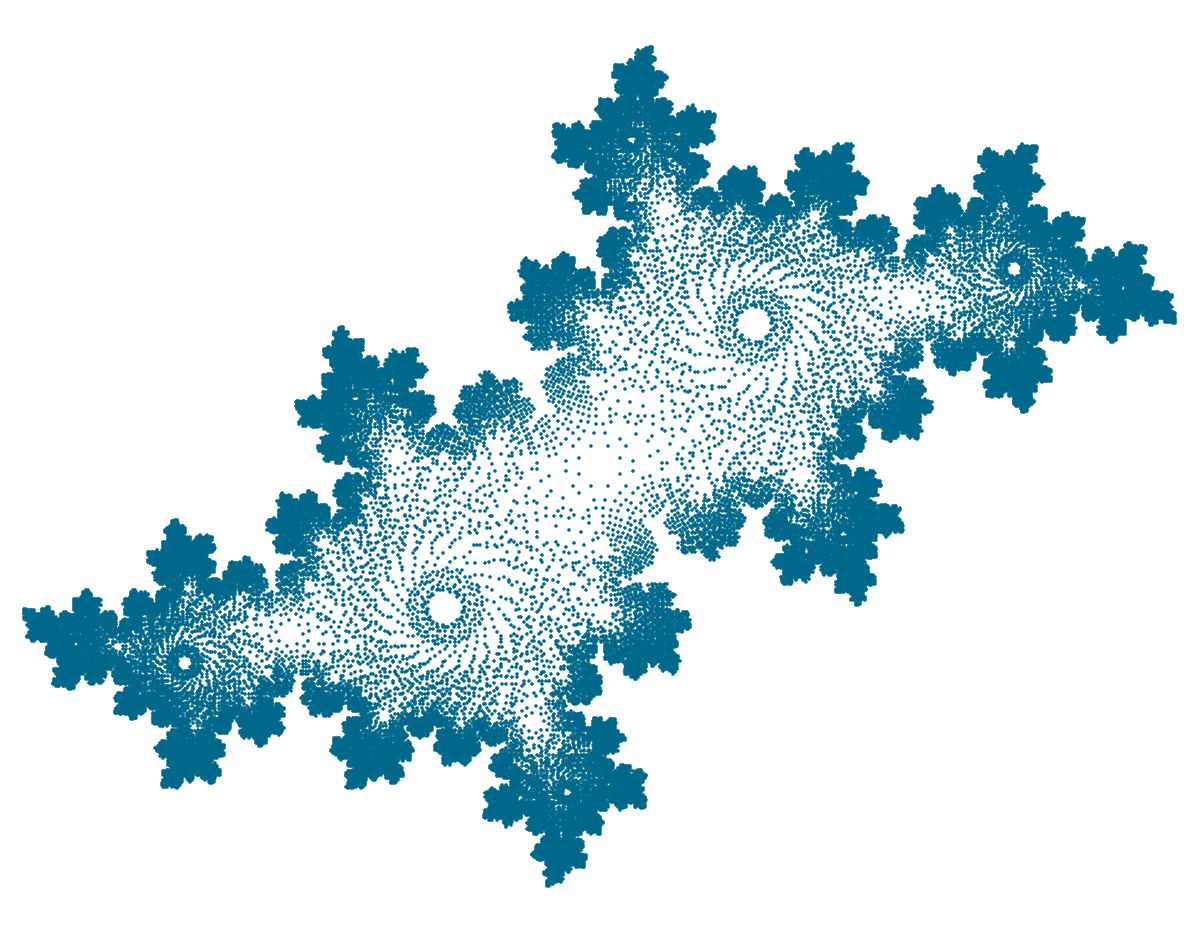
\includegraphics[scale=0.16]{julia2.png}
	
	\scriptsize
	    Julia set $c = -0.39 - 0.59 i$
}
\end{frame}

\section{Physics}
\subsection{Dummy}
\begin{frame}{Scaling}

\begin{itemize}
	\item Give a physical meaning $\rightarrow$ give a length scale

\begin{columns}
\newcommand{\s}{.2}
  \begin{column}{3cm}
  \centering
    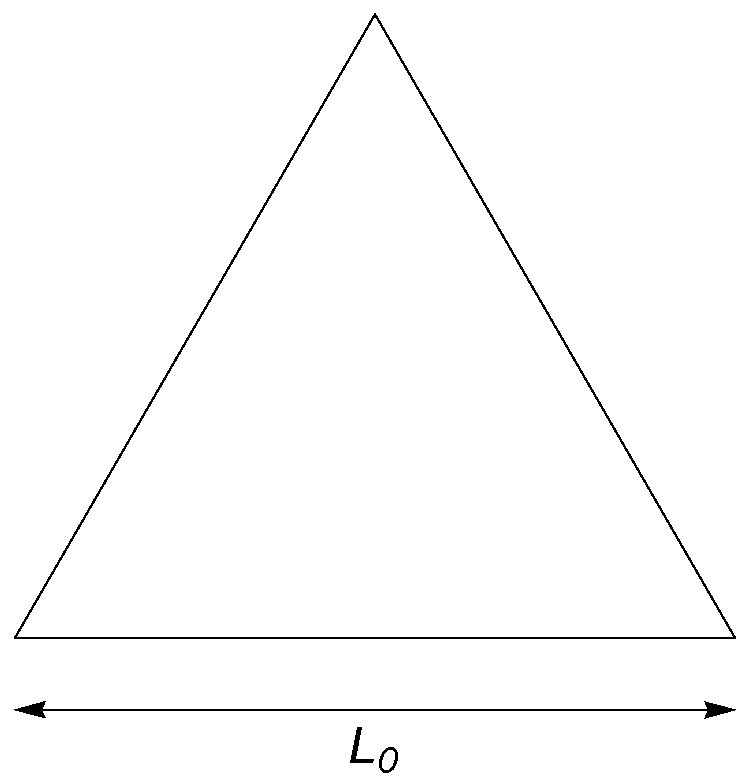
\includegraphics[scale=\s]{scale0.pdf}
  \end{column}

  \begin{column}{3cm}
  	\centering
     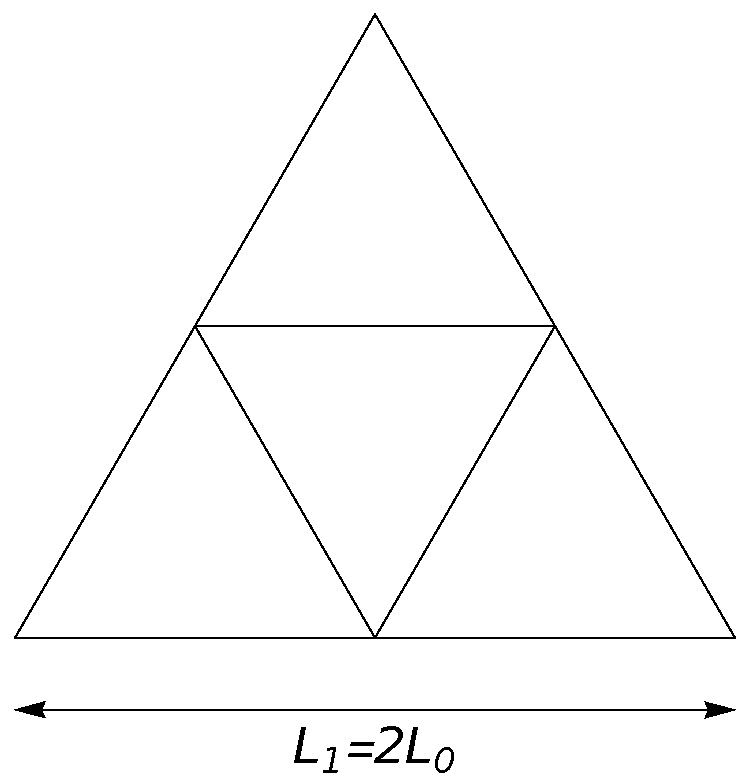
\includegraphics[scale=\s]{scale1.pdf}
  \end{column}
  
  \begin{column}{1cm}
  \centering
  ...
  \end{column}
  
    \begin{column}{3cm}
    \centering
    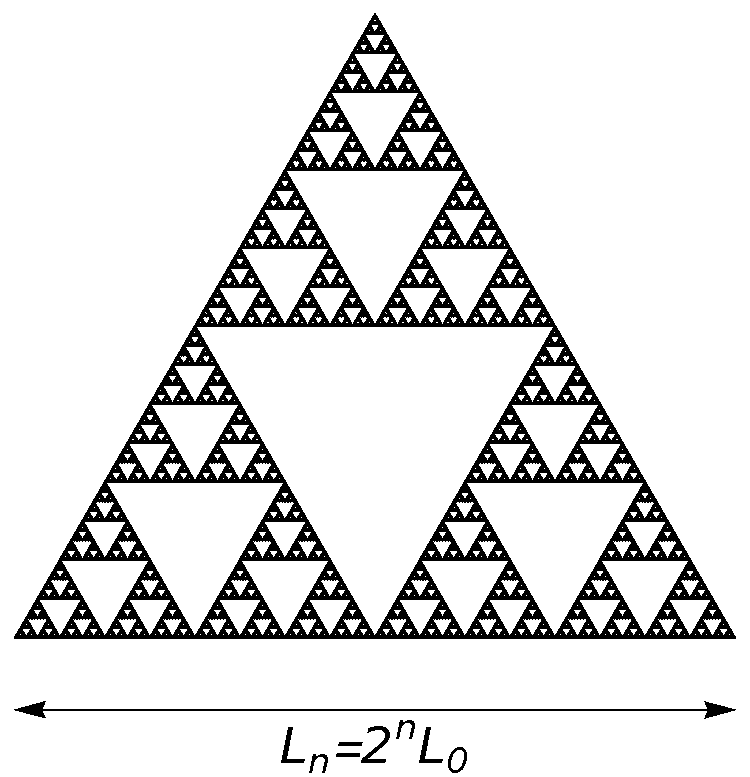
\includegraphics[scale=\s]{scaleInfty.pdf}
  \end{column}
\end{columns}

	\item A natural way of doing it:
	
	{\centering 
	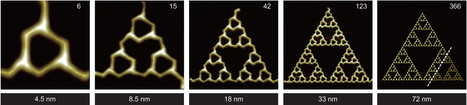
\includegraphics[scale=0.4]{sierpinsky_nature.jpg}
	\scriptsize
	
	Assembling molecular Sierpiński triangle fractals, Nature Chemistry (2015)
	
	}
	
	\item Scaling of physical quantities? 
	\begin{itemize}
		\item $M(L) \propto L^d$ on a $d$-dimensional Euclidean manifold... What happens on a fractal one?
	\end{itemize}
\end{itemize}
	
\end{frame}

\begin{frame}{The mass dimension}

\begin{itemize}
	\item $M(L) \propto L^d$ on a $d$-dimensional Euclidean manifold... What happens on a fractal one?

\begin{columns}
\newcommand{\s}{.2}
  \begin{column}{3cm}
  	\centering
    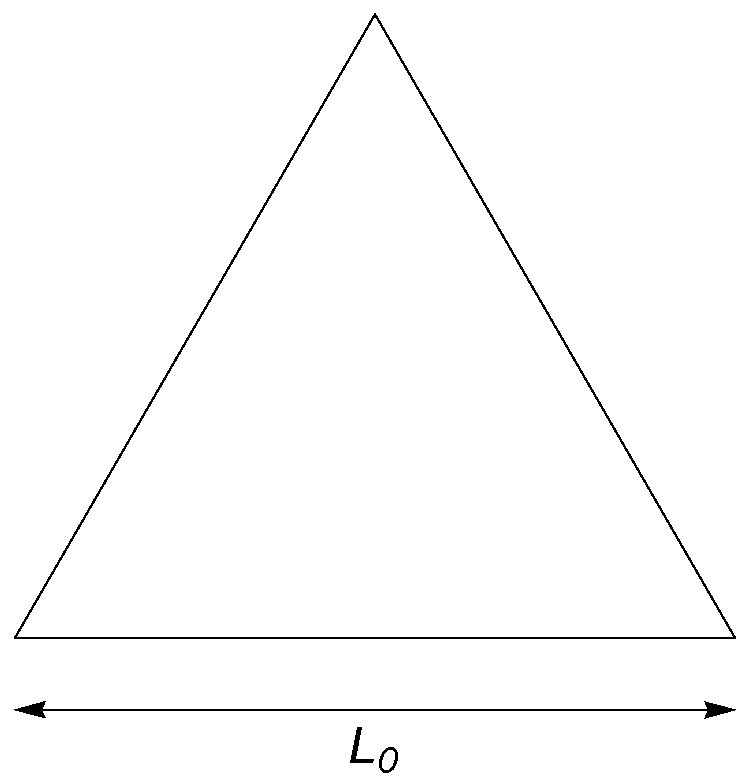
\includegraphics[scale=\s]{scale0.pdf}
    \scriptsize
    \[ M_0 \]
  \end{column}

  \begin{column}{3cm}
  	\centering
     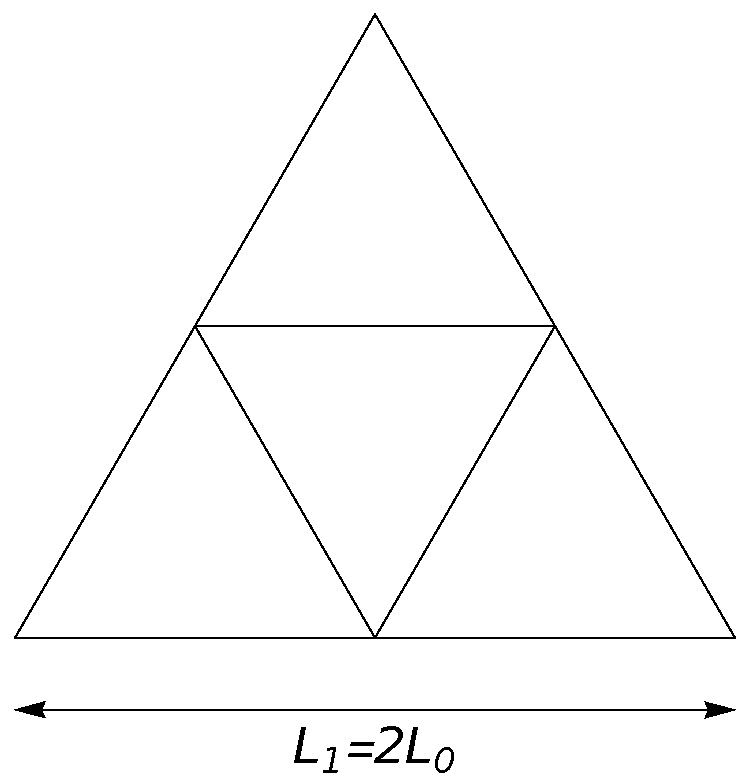
\includegraphics[scale=\s]{scale1.pdf}
     \scriptsize
    \[ M_1= 3M_0 \]
  \end{column}
  
  \begin{column}{1cm}
  \centering
  ...
  \end{column}
  
    \begin{column}{3cm}
    \centering
    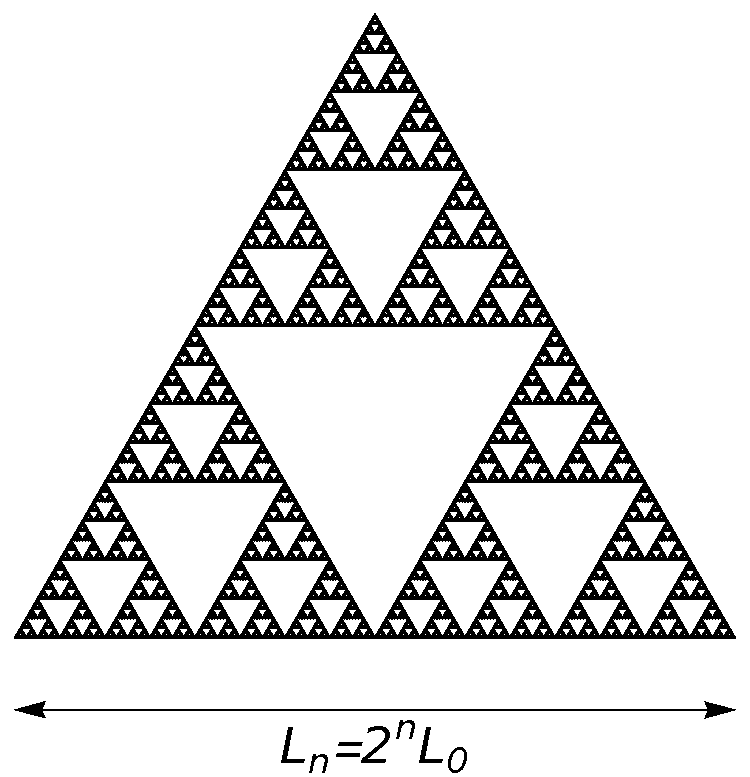
\includegraphics[scale=\s]{scaleInfty.pdf}
    \scriptsize
    \[ M_n= 3^nM_0 \]
  \end{column}
\end{columns}

\[ M(L) \propto L^{d_M} \text{, with } d_M = \log 3/\log 2 \]

	\item $d_M$ is the mass (or Hausdorff) dimension.
	
	\item $1 < d_M < 2$ different from $d = 1$, non-integer $\rightarrow$ signature of a fractal manifold.

\end{itemize}

\end{frame}

\begin{frame}

\begin{itemize}
\item Mass dimension: spot fractals, from large scales... 

	{\centering
    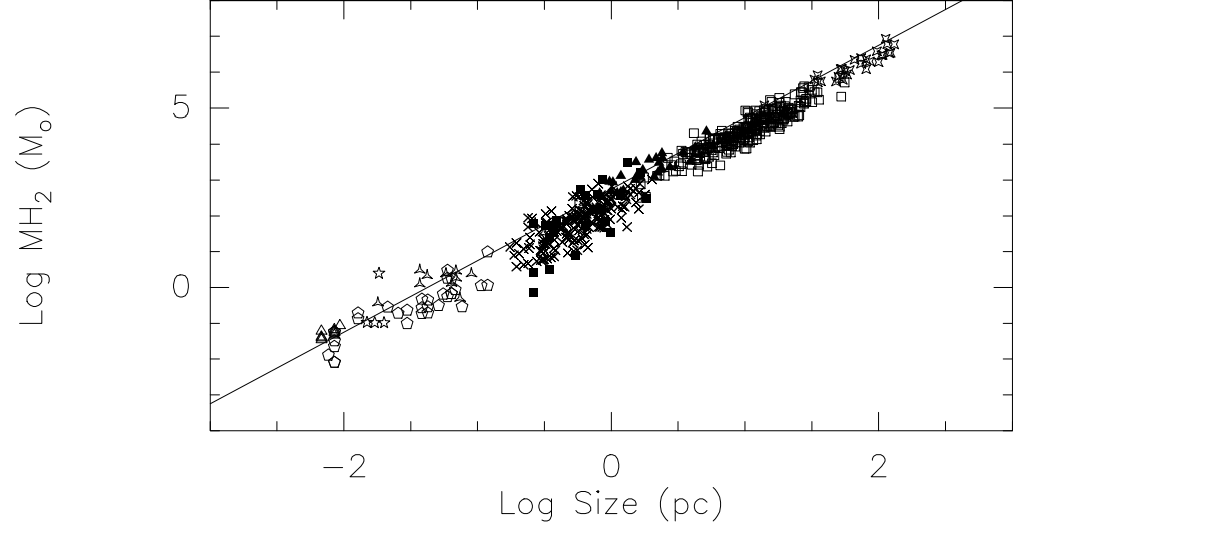
\includegraphics[scale=.18]{combes_interstellar_medium.png}
    \scriptsize
    
    Insterstallar medium fractal over 4 to 6 orders of magnitude [Fig.\ from Combes 1999]
    
    }
\item  ... to small ones

  	\centering
    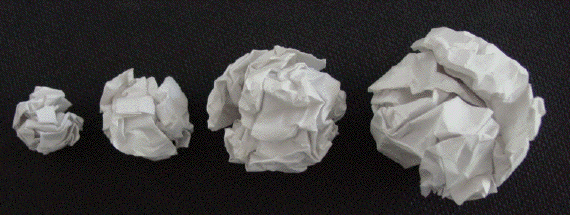
\includegraphics[scale=.3]{crumpled_paper.png}
    \scriptsize
\end{itemize}
\end{frame}

\begin{frame}{The electric dimension}
{\scriptsize [Akkermans, 2015 lectures]}
\begin{columns}
\newcommand{\s}{.2}
  \begin{column}{3cm}
  	\centering
    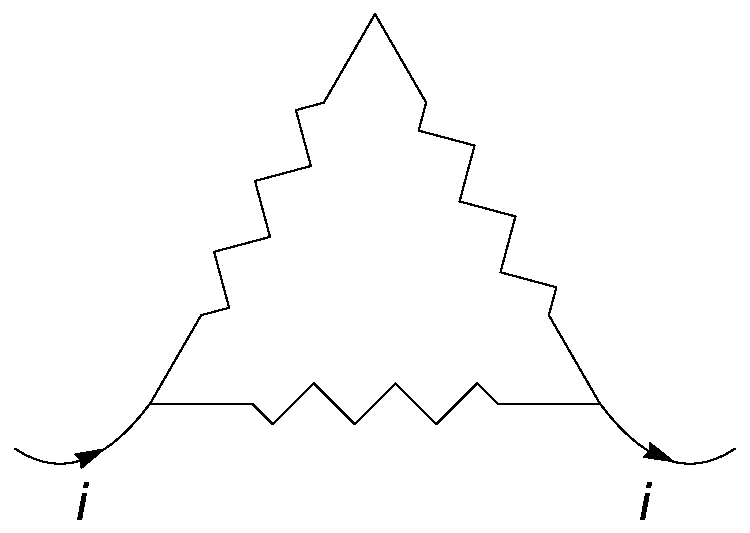
\includegraphics[scale=\s]{res0.pdf}
    \scriptsize
    \[ R_0 \]
  \end{column}

  \begin{column}{3cm}
  	\centering
     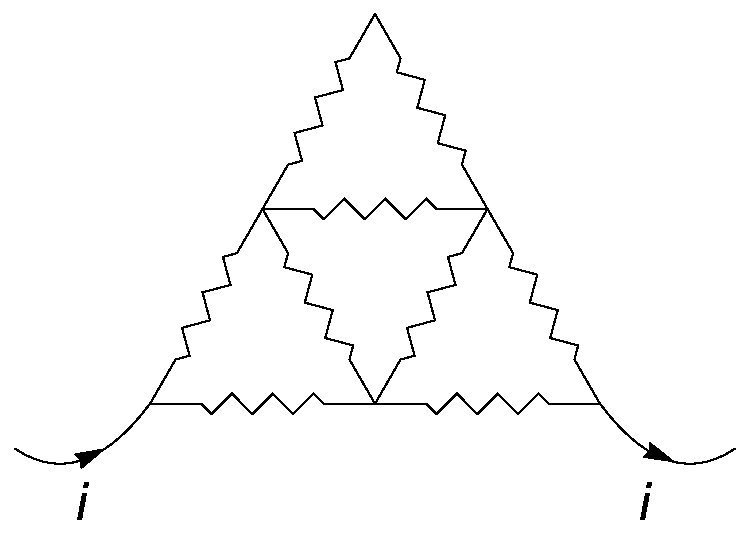
\includegraphics[scale=\s]{res1.pdf}
     \scriptsize
    \[ R_1= ? R_0 \]
  \end{column}
  
  \begin{column}{1cm}
  \centering
  ...
  \end{column}
  
    \begin{column}{3cm}
    \centering
    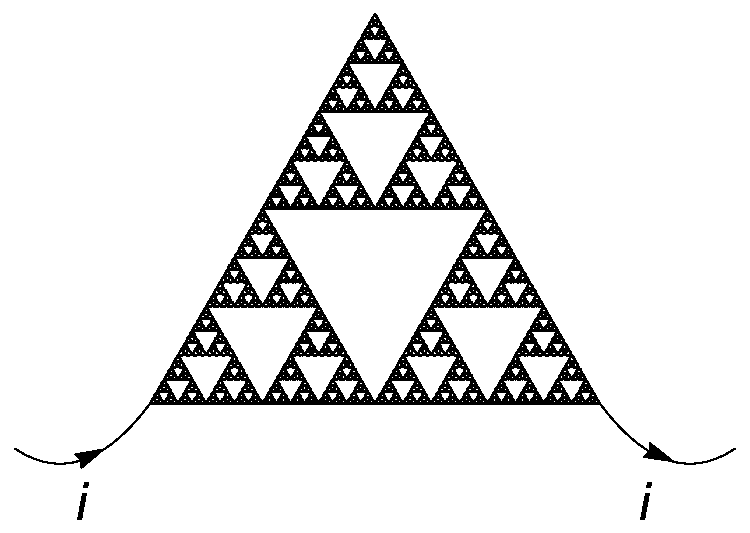
\includegraphics[scale=\s]{resInfty.pdf}
    \scriptsize
    \[ R_n= ?^nR_0 \]
  \end{column}
\end{columns}

\[ R(L) \propto L^{d_e} \text{, with } d_e = \log ?/\log 2 \]

\begin{itemize}
	\item $d_M \neq d_e$, both reflect the structure of the fractal manifold.
	\item On an Euclidean manifold $d_M = d_e = d$.
\end{itemize}

\end{frame}


\begin{frame}{The Fibonacci molecule}
    \begin{itemize}
    	\item The Fibonacci sequence: \\
    \only<1>{\textcolor{Complementary}{B}\\}
	\only<1>{\textcolor{BostonBlue}{A}\\}
	\only<1>{\textcolor{BostonBlue}{A}\textcolor{Complementary}{B}}
	\only<2>{\textcolor{Complementary}{A}\\}
	\only<2>{\textcolor{BostonBlue}{AB}\\}
	\only<2>{\textcolor{BostonBlue}{AB}\textcolor{Complementary}{A}}
	\only<3>{\textcolor{Complementary}{AB}\\}
	\only<3>{\textcolor{BostonBlue}{ABA}\\}
	\only<3>{\textcolor{BostonBlue}{ABA}\textcolor{Complementary}{AB}}
	\only<4>{\textcolor{Complementary}{ABA}\\}
	\only<4>{\textcolor{BostonBlue}{ABAAB}\\}
	\only<4>{\textcolor{BostonBlue}{ABAAB}\textcolor{Complementary}{ABA}}
	\only<5>{\textcolor{Complementary}{ABAAB}\\}
	\only<5>{\textcolor{BostonBlue}{ABAABABA}\\}
	\only<5>{\textcolor{BostonBlue}{ABAABABA}\textcolor{Complementary}{ABAAB}}
	\only<6>{\textcolor{Complementary}{ABAABABA}\\}
	\only<6>{\textcolor{BostonBlue}{ABAABABAABAAB}\\}
	\only<6>{\textcolor{BostonBlue}{ABAABABAABAAB}\textcolor{Complementary}{ABAABABA}}
	\only<7>{\textcolor{Complementary}{ABAABABAABAAB}\\}
	\only<7>{\textcolor{BostonBlue}{ABAABABAABAABABAABABA}\\}
	\only<7>{\textcolor{BostonBlue}{ABAABABAABAABABAABABA}\textcolor{Complementary}{ABAABABAABAAB}}
	
	\item The Fibonacci molecule:
	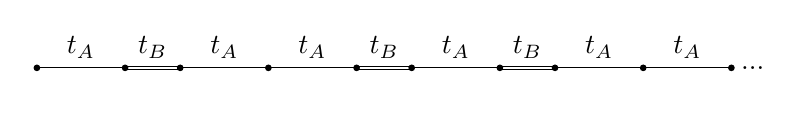
\begin{tikzpicture}[scale=.7]
	    		\newcommand{\orig}{-1.5}
    		\newcommand{\tA}{1.6}
    		\newcommand{\tB}{1.}
    		\newcommand{\vertspac}{-2.}
    	
    		% initial chain
    	
    		% bonds 
        	\draw[-] (\orig,0) -- (\orig+\tA,0) node [midway, above] {$t_A$};
        	\draw[-,double] (\orig+\tA,0) -- (\orig+\tA+\tB,0) node [midway, above] {$t_B$};
			\draw[-] (\orig+\tA+\tB,0) -- (\orig+2*\tA+\tB,0) node [midway, above] {$t_A$};	
			\draw[-] (\orig+2*\tA+\tB,0) -- (\orig+3*\tA+\tB,0) node [midway, above] {$t_A$};
			\draw[-,double] (\orig+3*\tA+\tB,0) -- (\orig+3*\tA+2*\tB,0) node [midway, above] {$t_B$};
			\draw[-] (\orig+3*\tA+2*\tB,0) -- (\orig+4*\tA+2*\tB,0) node [midway, above] {$t_A$};
			\draw[-,double] (\orig+4*\tA+2*\tB,0) -- (\orig+4*\tA+3*\tB,0) node [midway, above] {$t_B$};
			\draw[-] (\orig+4*\tA+3*\tB,0) -- (\orig+5*\tA+3*\tB,0) node [midway, above] {$t_A$};
			\draw[-] (\orig+5*\tA+3*\tB,0) -- (\orig+6*\tA+3*\tB,0) node [midway, above] {$t_A$};
    	
    	
    		% sites
		    \filldraw (\orig,0) circle (0.05) node [below] {};
		    \filldraw (\orig+\tA,0) circle (0.05) node [below] {};
		    \filldraw (\orig+\tA+\tB,0) circle (0.05) node [below] {};
		    \filldraw (\orig+2*\tA+\tB,0) circle (0.05) node [below] {};
		    \filldraw (\orig+3*\tA+\tB,0) circle (0.05) node [below] {};
		    \filldraw (\orig+3*\tA+2*\tB,0) circle (0.05) node [below] {};
		    \filldraw (\orig+4*\tA+2*\tB,0) circle (0.05) node [below] {};
		    \filldraw (\orig+4*\tA+3*\tB,0) circle (0.05) node [below] {};
		    \filldraw (\orig+5*\tA+3*\tB,0) circle (0.05) node [right] {};
		    \filldraw (\orig+6*\tA+3*\tB,0) circle (0.05) node [right] {...};
		      

	\end{tikzpicture}
	\item The molecule is \textbf{not} a fractal!
	\item A quantity of interest: molecular spectrum
	\end{itemize}
\end{frame}

\begin{frame}{Spectrum of Fibonacci molecules}
	\only<1>{\tiny\textcolor{BostonBlue}{AB}\textcolor{Complementary}{AABABAABAABABAABABAABAABABAABAABABAABABAABAABABAABABAABAABABAABAABABAABABAABAABABAABAAB}}
	\only<2>{\tiny\textcolor{BostonBlue}{ABA}\textcolor{Complementary}{ABABAABAABABAABABAABAABABAABAABABAABABAABAABABAABABAABAABABAABAABABAABABAABAABABAABAAB}}
	\only<3>{\tiny\textcolor{BostonBlue}{ABAAB}\textcolor{Complementary}{ABAABAABABAABABAABAABABAABAABABAABABAABAABABAABABAABAABABAABAABABAABABAABAABABAABAAB}}
	\only<4>{\tiny\textcolor{BostonBlue}{ABAABABA}\textcolor{Complementary}{ABAABABAABABAABAABABAABAABABAABABAABAABABAABABAABAABABAABAABABAABABAABAABABAABAAB}}
	\only<5>{\tiny\textcolor{BostonBlue}{ABAABABAABAAB}\textcolor{Complementary}{ABAABABAABAABABAABAABABAABABAABAABABAABABAABAABABAABAABABAABABAABAABABAABAAB}}
	\only<6>{\tiny\textcolor{BostonBlue}{ABAABABAABAABABAABABA}\textcolor{Complementary}{ABAABABAABAABABAABABAABAABABAABABAABAABABAABAABABAABABAABAABABAABAAB}}
	\only<7>{\tiny\textcolor{BostonBlue}{ABAABABAABAABABAABABAABAABABAABAAB}\textcolor{Complementary}	{ABAABABAABAABABAABABAABAABABAABAABABAABABAABAABABAABAAB}}
	\only<8>{\tiny\textcolor{BostonBlue}{ABAABABAABAABABAABABAABAABABAABAABABAABABAABAABABAABABA}\textcolor{Complementary}{ABAABABAABAABABAABABAABAABABAABAAB}}
	\only<9>{\tiny\textcolor{BostonBlue}{ABAABABAABAABABAABABAABAABABAABAABABAABABAABAABABAABABAABAABABAABAABABAABABAABAABABAABAAB}
	\textcolor{Complementary}{~}
	}
	
	{
	\centering
	\only<1>{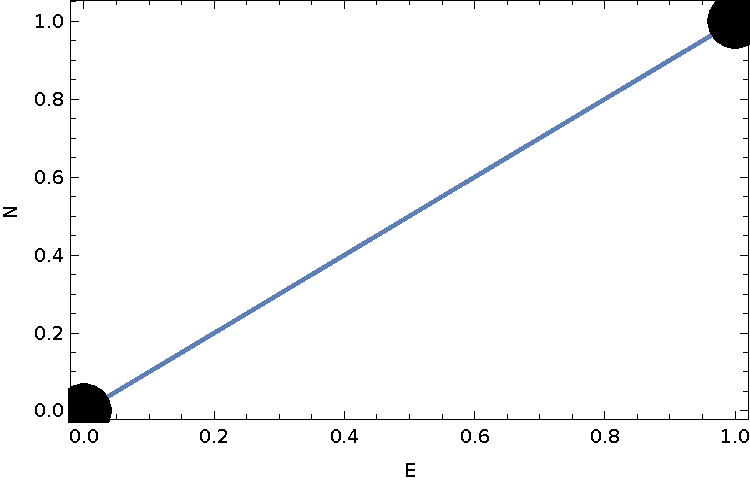
\includegraphics[width=0.7\textwidth]{idos_3}}
	\only<2>{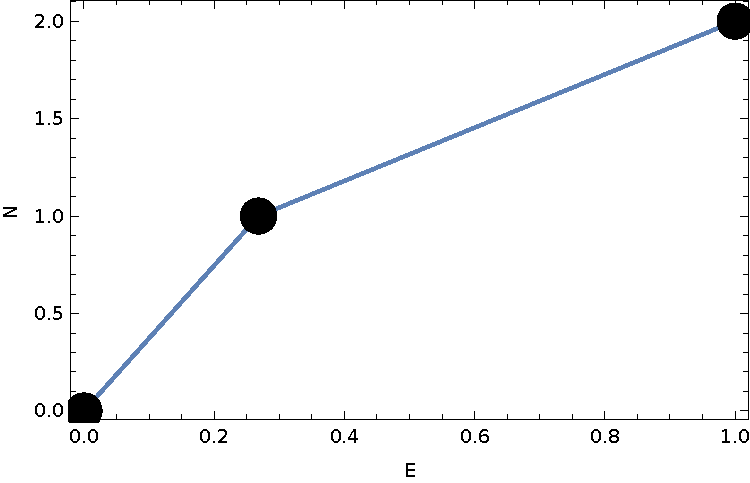
\includegraphics[width=0.7\textwidth]{idos_4}}
	\only<3>{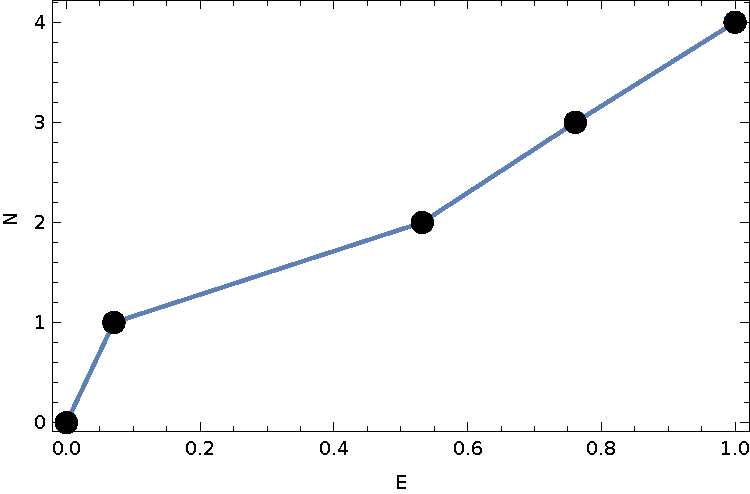
\includegraphics[width=0.7\textwidth]{idos_5}}
	\only<4>{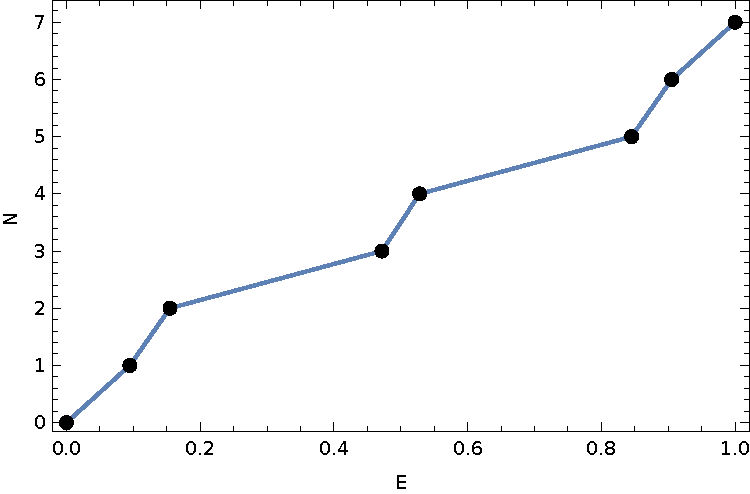
\includegraphics[width=0.7\textwidth]{idos_6}}
	\only<5>{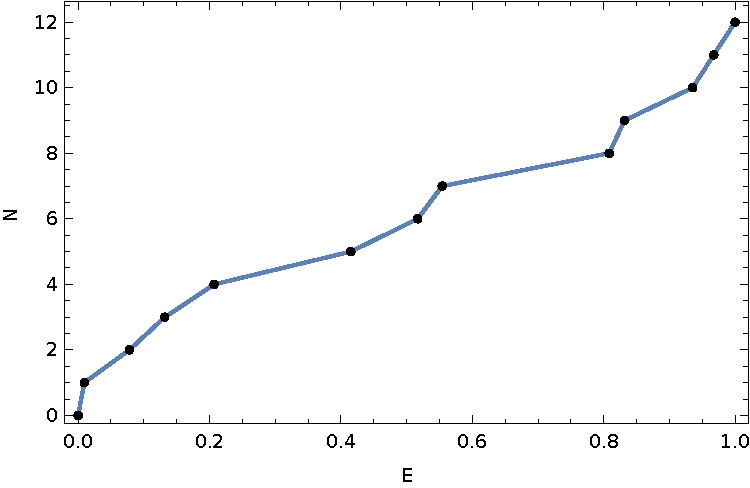
\includegraphics[width=0.7\textwidth]{idos_7}}
	\only<6>{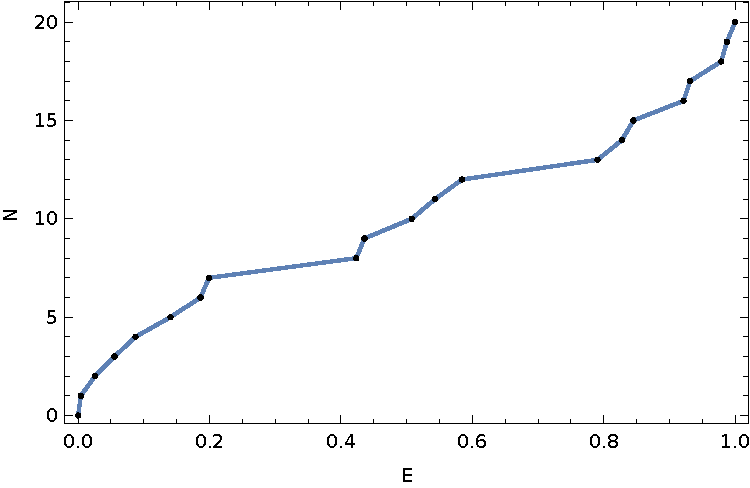
\includegraphics[width=0.7\textwidth]{idos_8}}
	\only<7>{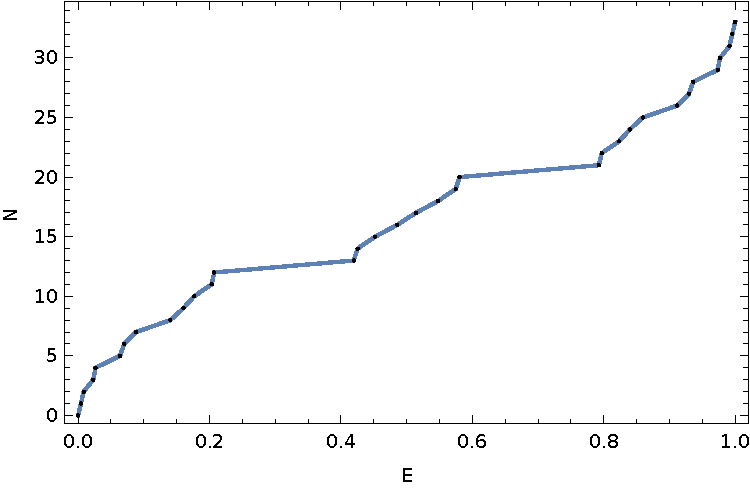
\includegraphics[width=0.7\textwidth]{idos_9}}
	\only<8>{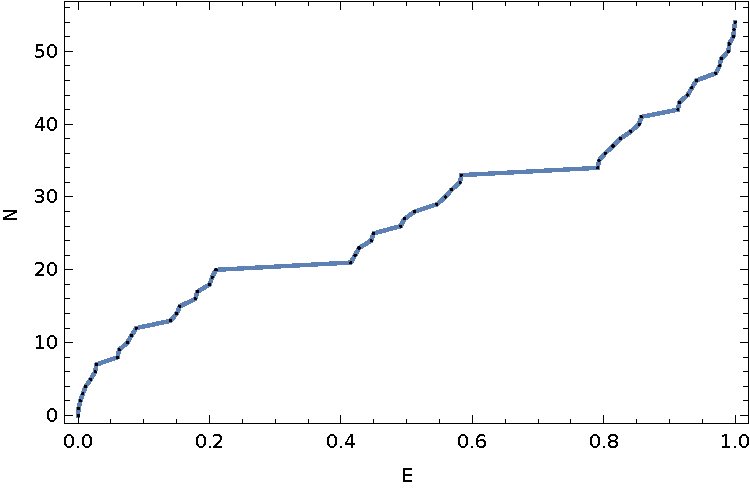
\includegraphics[width=0.7\textwidth]{idos_10}}
	\only<9>{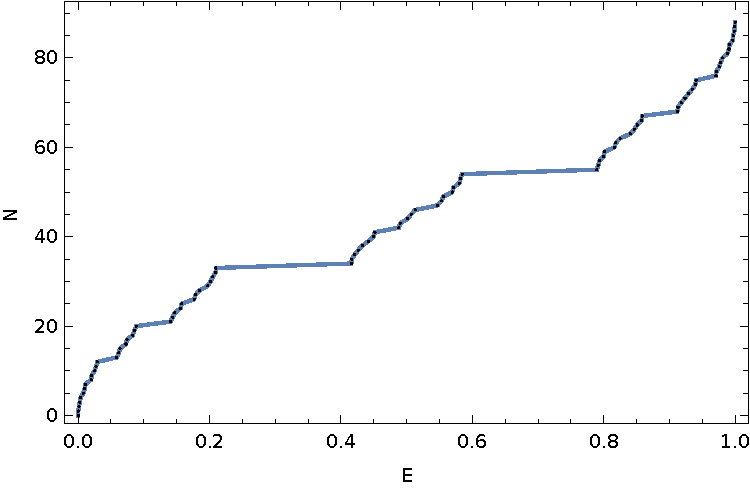
\includegraphics[width=0.7\textwidth]{idos_11}}
	
	}
\end{frame}
	
\begin{frame}{Hidden fractals: the Fibonacci chain}

	\begin{itemize}
	\item No obvious fractal nature, but...
    \end{itemize}
     {\centering
    	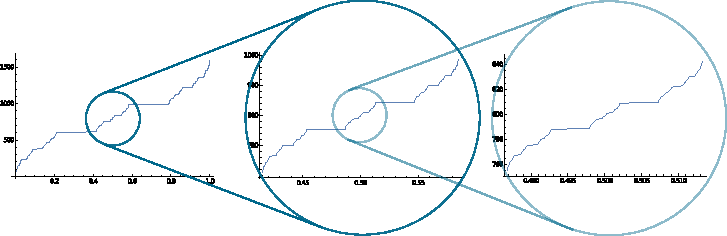
\includegraphics[scale=.9]{idos.pdf}
    	
     }
     ... the graph of the density of states is a fractal!
     
     \begin{itemize}
     	\item What can we say about a scale invariant function?
      \end{itemize}
	
\end{frame}

\begin{frame}{Interlude: discrete and continuous scale invariance}
    \begin{columns}
\newcommand{\s}{.2}
  \begin{column}{5cm}
  	\begin{block}{\textcolor{BostonBlue}{Continuous} scale invariance}
  	\begin{align*}
		\textcolor{BostonBlue}{\forall a},~ f(ax) &= b(a) f(x) \\
		\text{Then } f(x) &= C x^\alpha
	\end{align*}
  	\end{block}
  \end{column}

  \begin{column}{5cm}
  	\begin{block}{\textcolor{Complementary}{Discrete} scale invariance}
  	\begin{align*}
		\textcolor{Complementary}{\exists a},~ f(ax) &= b(a) f(x) \\
		\text{Then } f(x) &= ?
	\end{align*}
  	\end{block}
  \end{column}
\end{columns}

\[
	f(x) = G\left(\frac{\ln x}{\ln a}\right) x^\alpha~\text{\scriptsize [Saleur, Sornette 1996]}
\]

First order expansion:
\[
	f(x) \simeq \left[G_0 + G_1 \cos\left(2 \pi \frac{\ln x}{\ln a}\right)\right] x^\alpha
\]
$\rightarrow$ \textbf{log-periodic oscillations}
\end{frame}

\begin{frame}{Fibonacci and $\log$--periodic oscillations}
		\centering
		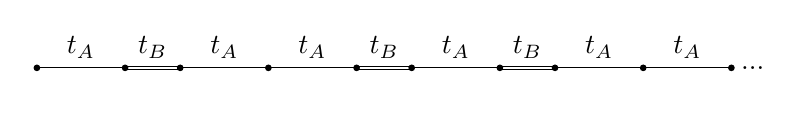
\begin{tikzpicture}[scale=.7]
	    		\newcommand{\orig}{-1.5}
    		\newcommand{\tA}{1.6}
    		\newcommand{\tB}{1.}
    		\newcommand{\vertspac}{-2.}
    	
    		% initial chain
    	
    		% bonds 
        	\draw[-] (\orig,0) -- (\orig+\tA,0) node [midway, above] {$t_A$};
        	\draw[-,double] (\orig+\tA,0) -- (\orig+\tA+\tB,0) node [midway, above] {$t_B$};
			\draw[-] (\orig+\tA+\tB,0) -- (\orig+2*\tA+\tB,0) node [midway, above] {$t_A$};	
			\draw[-] (\orig+2*\tA+\tB,0) -- (\orig+3*\tA+\tB,0) node [midway, above] {$t_A$};
			\draw[-,double] (\orig+3*\tA+\tB,0) -- (\orig+3*\tA+2*\tB,0) node [midway, above] {$t_B$};
			\draw[-] (\orig+3*\tA+2*\tB,0) -- (\orig+4*\tA+2*\tB,0) node [midway, above] {$t_A$};
			\draw[-,double] (\orig+4*\tA+2*\tB,0) -- (\orig+4*\tA+3*\tB,0) node [midway, above] {$t_B$};
			\draw[-] (\orig+4*\tA+3*\tB,0) -- (\orig+5*\tA+3*\tB,0) node [midway, above] {$t_A$};
			\draw[-] (\orig+5*\tA+3*\tB,0) -- (\orig+6*\tA+3*\tB,0) node [midway, above] {$t_A$};
    	
    	
    		% sites
		    \filldraw (\orig,0) circle (0.05) node [below] {};
		    \filldraw (\orig+\tA,0) circle (0.05) node [below] {};
		    \filldraw (\orig+\tA+\tB,0) circle (0.05) node [below] {};
		    \filldraw (\orig+2*\tA+\tB,0) circle (0.05) node [below] {};
		    \filldraw (\orig+3*\tA+\tB,0) circle (0.05) node [below] {};
		    \filldraw (\orig+3*\tA+2*\tB,0) circle (0.05) node [below] {};
		    \filldraw (\orig+4*\tA+2*\tB,0) circle (0.05) node [below] {};
		    \filldraw (\orig+4*\tA+3*\tB,0) circle (0.05) node [below] {};
		    \filldraw (\orig+5*\tA+3*\tB,0) circle (0.05) node [right] {};
		    \filldraw (\orig+6*\tA+3*\tB,0) circle (0.05) node [right] {...};
		      

	\end{tikzpicture}

	\begin{columns}
	\begin{column}{0.5\textwidth}
	{\centering
    	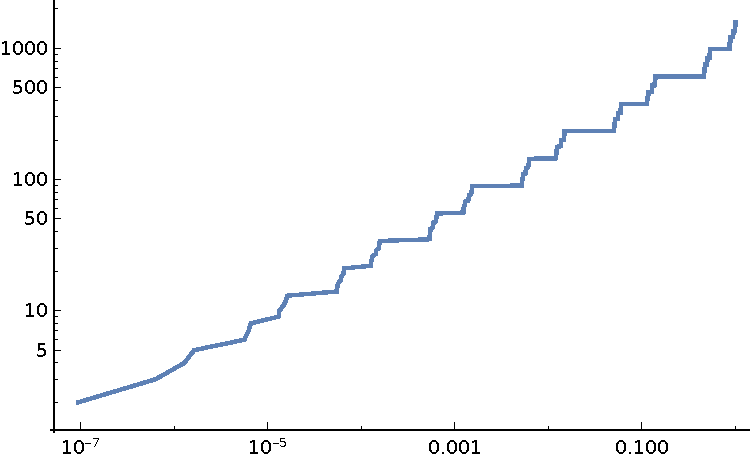
\includegraphics[width=\columnwidth]{idoslog.pdf}
    	
    	    	    	\scriptsize
		Spectrum of the molecule
    	
    }
    \end{column}
    \begin{column}{0.5\textwidth}
	{\centering
    	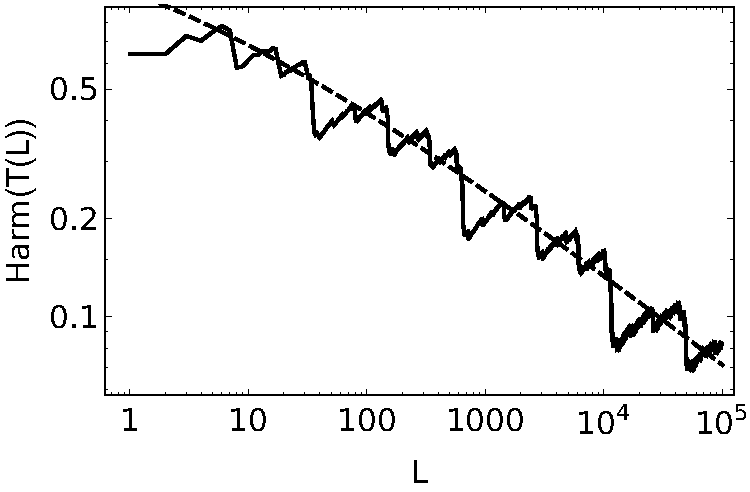
\includegraphics[width=\columnwidth]{harmonic_mean_transmission}
    	
    	    	\scriptsize
		Transmission probability
		[Macé \emph{et al} 2017]
			
    }
    \end{column}
    \end{columns}
\end{frame}

\section{Summary}
\subsection{Dummy}

\begin{frame}{Fractals:}
    \begin{itemize}
        \item break continuous scaling symmetry into discrete
        \item are rough objects, mathematically interesting
        \item arise in surprisingly diverse areas of physics
        \item ... and, always, are beautiful!
    \end{itemize}
    
     {\centering
    	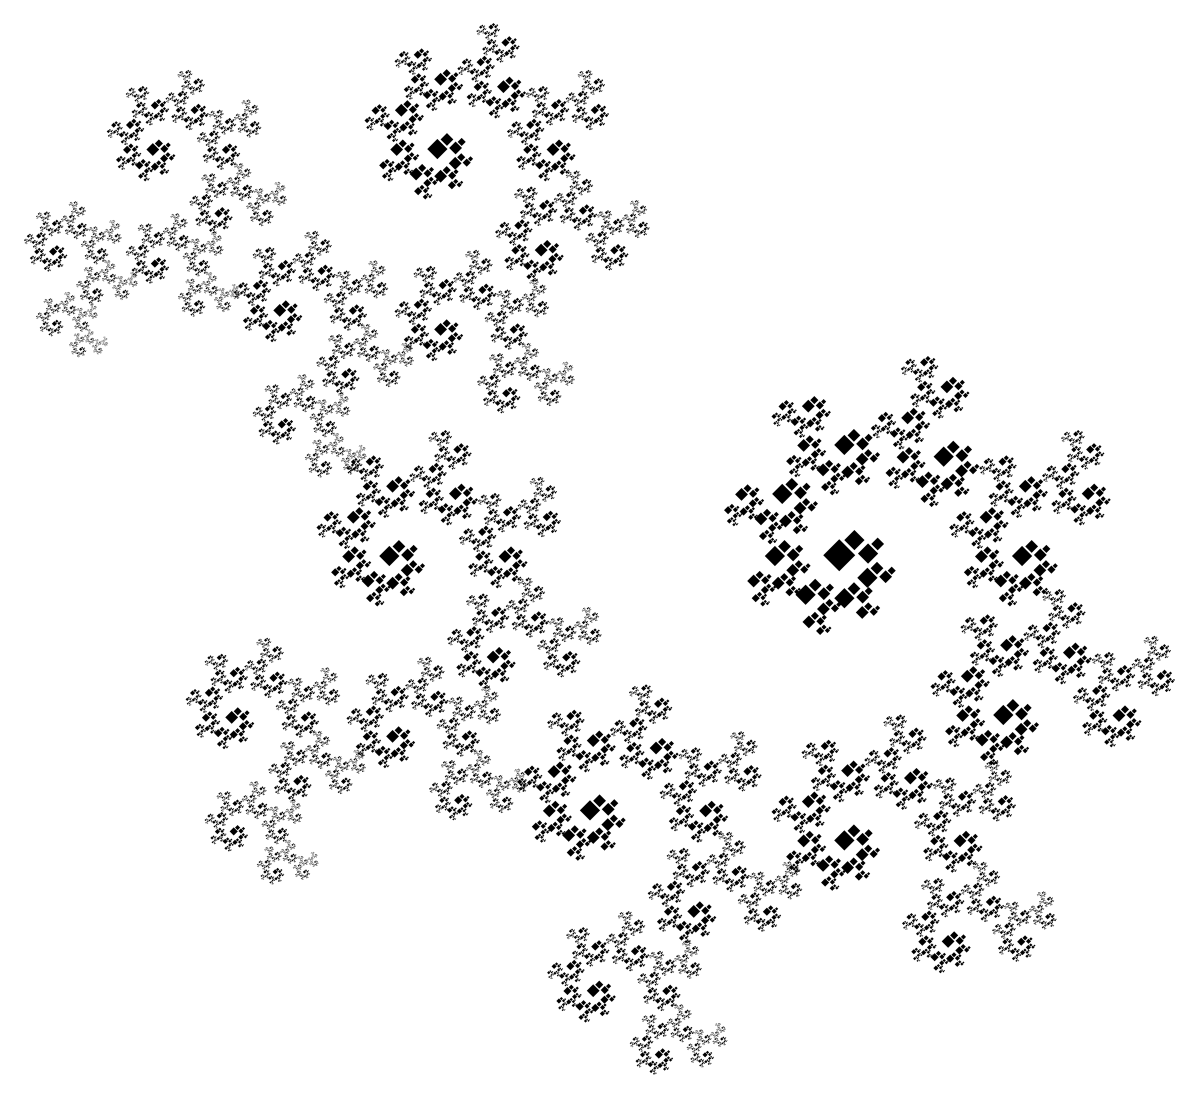
\includegraphics[scale=.14]{dragon.png}
    	
     }
\scriptsize
[Slides and scripts: \href{https://github.com/Yukee/talks/}{github.com/Yukee/talks}]
\end{frame}

\end{document}
